\chapter{Discussion}

\section{Comparison with real EEG Data during Propofol-Sedation}

\begin{figure}[H]
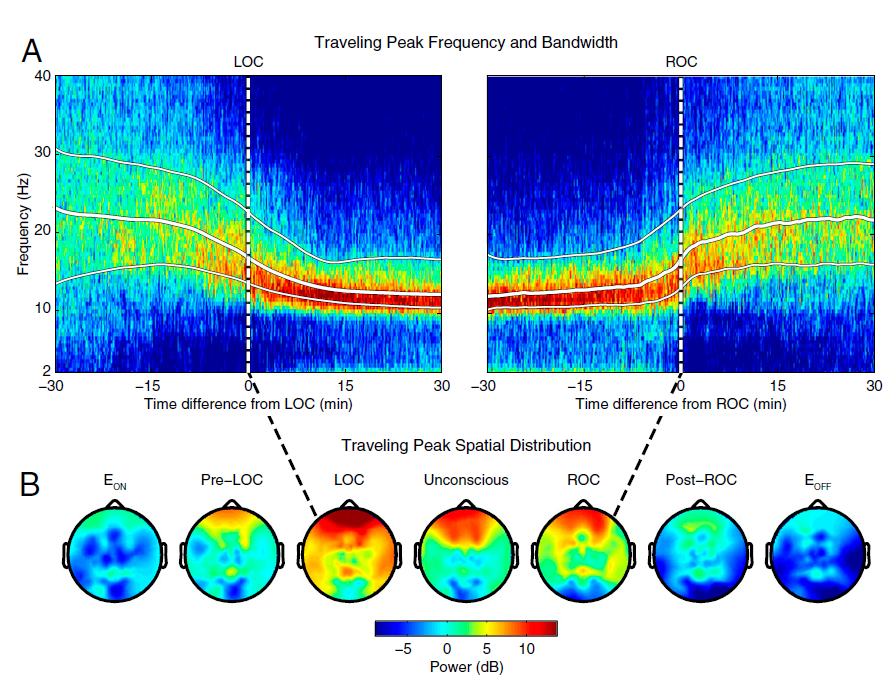
\includegraphics[width=15cm]{Figures/purdon2.png}
\caption{\textbf{Real EEG Data \cite{purdon_electroencephalogram_2013}:} Traveling Peak and general shift of Spectral Power from above 20 to the 10Hz Range during sedation. Also note the power increase in the very slow frequencies.}
\end{figure}

\quad\todo{compare to Purdon \cite{purdon_electroencephalogram_2013}, Lee \cite{lee_classification_2017}}

\section{Outlook}

\quad\todo{how this could be extended towards our goal (include thalamus like in COALIA, find ways to simulate TBI-induced DOC more specifically, create combination of conditions and states of awareness in the same model, ...)}